\section{Results}
This section will present and analyze the results from the described experiments 
and will be addressed similarly to that structure. However, first, the baseline 
will be tested in each environment in order to establish the complexity of the 
environments beforehand. 

\subsection{Hardware}
The experiments have been performed on a NVIDIA Geforce GTX 980M graphics card, 
with 8GB of RAM and an Intel Core i7-4720HQ CPU with 2.60GHz. The simulation uses a mix 
of both the GPU and the CPU in order to perform the basic operations. The RL framework 
relied solely on the CPU in order to allow the rest of the GPU space to be used for the 
training of the agent. 

\subsection{Baseline Performance}
The initial tests will first be performed by a baseline 
agent. This agent has been run in each environment, in order to see how it performs and 
behaves. The same metrics as for the RL agents will be recorded, and these values 
will be used as a measuring tool for the RL agents. More specifically, the 
degradation in performance with the previous environment will be calculated. After 
having run the tests, these results can be seen in Figure \ref{tab:BaselinesAVG}.

\begin{table}[h]
    \centering
    \caption{Average return of the baseline agent in each environment and the corresponding 
    degradation of performance compared to the previous environment}
    \label{tab:BaselinesAVG}
    \begin{tabular}{l|c|c}
    \multicolumn{1}{c|}{\textbf{Environment}} & \textbf{Average Return (/50)} & \textbf{Difference*} \\ \hline
    BlocksNormal    & 40.2 & -        \\
    BlocksObstacles & 22.9  & -43.0 \% \\
    Factory   & 9.9  & -56.8 \%
    \end{tabular}
    \justify
    \small
    *The difference has been calculated by comparing the average return of an agent with 
    the average return in the previous environment. 
\end{table}

What can be deduced from these initial results, is that the baseline agent 
has more trouble the more obstacles are being added to the environment. With 
the addition of walls in the BlocksObstacles environment, the agent already 
performs considerably worse. However, what becomes clear, is that the
implementation of the agent in an even more complex environment, results in 
an even bigger performance drop. These findings more strongly emphasize 
the weaknesses of baseline implementations: namely their inability to 
deal with obstacles and complex environments. 

In order to further 
investigate how an average episodes is performed by the baseline, a 
reward distribution has been created, as seen in Figure \ref{im:BaselinesDistros}. 
Here the proportion of time that a positive reward signal was received at a 
given step in the episode has been plotted, with the green line representing 
a running average of the last 5 steps. 

\begin{Figure}
    \centering
    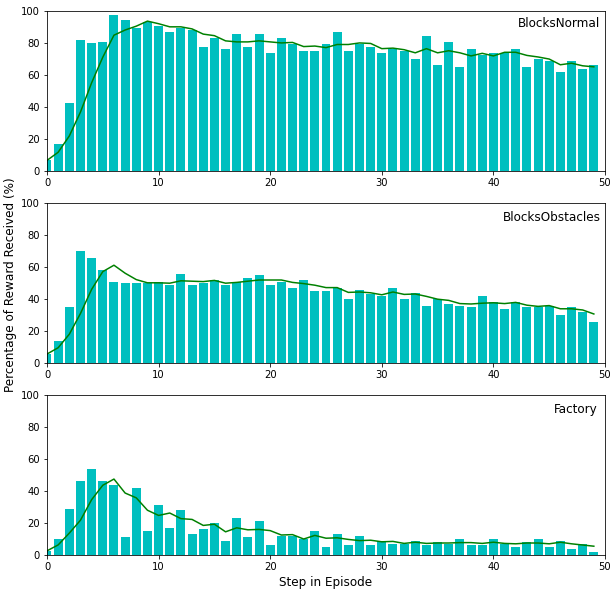
\includegraphics[width=0.8\linewidth]{results/Reward Distribution of Baselines.png}
    \captionof{figure}{Baseline reward distributions in each environment}
    \label{im:BaselinesDistros}
\end{Figure}

The first five frames of an average episode look the same for each agent. This is 
reflected in the image by the sharp increase in reward early in the episode. 
During the first frames, it is hard for the agent to receive  
reward because of the reset distance between the drone and the person. 
Reflected in the figure, the beginning frames contain low values. This 
lack of reward in the initial steps is also the explanation for why the agent 
will never be able to receive an average reward of 50, as receiving a reward 
in these initial steps is extremely hard. The consequent steps,
however, increase drastically, seeing as the drone is approaching the person. 
This behavior happens in each episode because in the first moments, the chances 
that the person will have walked behind an obstacle are slim, resulting in these moments 
where the agent is able to follow. Nonetheless,
it is still very hard to maintain a 100\% reward in each consequent step, as the agent 
sometimes acts slightly too late, resulting in some steps where no reward is received. 
This same pattern is visible in two obstacle environment, however with a proportional 
degradation in rewards in the later stages. This points at the inability of this 
agent to avoid obstacles after the initial run-up to the person. 

\begin{Figure}
    \centering
    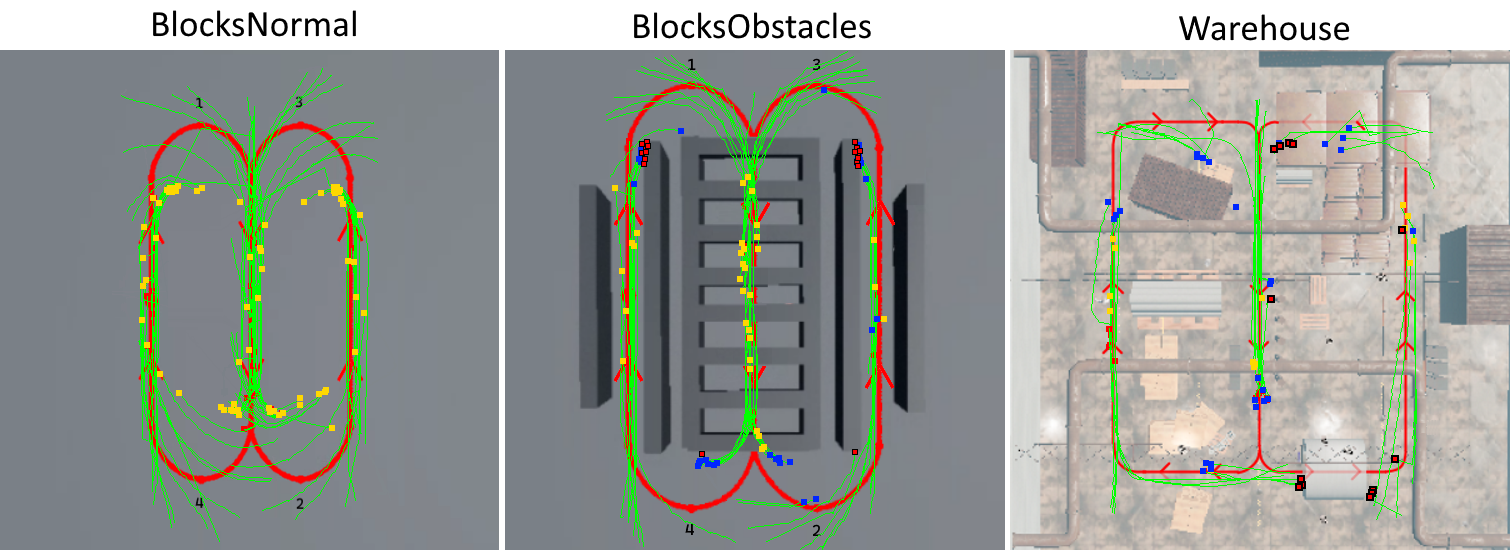
\includegraphics[width=\linewidth]{results/BaselineEnvironmentsPaths.png}
    \tiny 
    Yellow = Normal end $|$ Blue = Out of View $|$ Red = Collision
    \captionof{figure}{Paths and episode ends of the baseline ends during 100 episode test runs 
    for each environment}
    \label{im:BaselinePaths}
\end{Figure}

Looking at the path of the baseline inside of the BlocksNormal environment in 
Figure \ref{im:BaselinePaths}, 
it is clear that the agent follows the paths of the person neatly. During 
the turns, the paths of the agent finds itself inside of the diameter of the 
turn, which is to be expected since in these moments all the agent 
needs to do is simply turn to keep the person in its FoV with the sporadic 
move forward in order to keep the person at the right distance. However, performing 
this behavior inside of the other two environments posed problems for
this agent as can be seen by the increase of collisions and moments of losing 
the person further illustrated by Table \ref{tab:BaselinesEnds}

\begin{table}[h]
    \centering
    \caption{Unsuccessful episode endings of the baseline in each environment during the test run}
    \label{tab:BaselinesEnds}
    \begin{tabular}{l|c|c|c}
    \multicolumn{1}{c|}{\textbf{Episode End Type}} & \textbf{BlocksNormal} & \textbf{BlocksObstacles} & \textbf{Warehouse} \\ \hline
    Out of View           & 0          & 33          & 16          \\
    Collisions            & 0          & 20          & 60          \\ \hline
    \textbf{Total (/100)} & \textbf{0} & \textbf{68} & \textbf{76}
    \end{tabular}
\end{table}

Looking at both 
types of hallways that the agent finds itself, it does not seem to struggle with 
these situations. Both the tight hallways on the outer sides of the walking route
and the wider hallway in the middle of the map, seem to be easy situations for 
the baseline to handle. This makes sense, as the baseline is programmed to simply 
move forward in these situations. It is the corners situation 
where this agent is unable perform adequately. There 
are four clusters where these problems seem to arise. Two at the bottom at the 
beginning of the turn, where the agent keeps losing sight of the person, and two at 
the top where the drone keeps crashing into the wall as well as lose sight of the 
person. Why the agent struggles in these situations is an expression of the fact 
that in these turns, it is necessary to be able to avoid an obstacle. Such behavior 
is not programmed, resulting in failing situations. An example of a failing moment 
can be seen in Figure \ref{im:BaselineLostSight}.\newline

\begin{Figure}
    \centering
    \small
    Image: view of the drone $|$ Arrows: Action the agent performed
    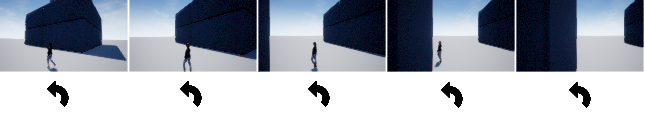
\includegraphics[width=\linewidth]{results/specific_situations/baseline_outofview.png}
    \captionof{figure}{How the baseline loses sight of the person in BlocksObstacle}
    \label{im:BaselineLostSight}
\end{Figure}

Since the person is within the correct distance, the agent does not come closer but 
instead keeps centering the person in its view. However, as can be seen in the last 
three frames, the wall is becoming visible. This does not influence its 
behavior, leading to the person walking behind the wall which makes the drone 
lose sight of the person. The reason why the collisions occur in the 
top two clusters, has to do with the type of situation the drone is in. In the top two 
turns, the drone is leaving tight hallways, where there is less room for mistakes leading 
to early collisions. This is less of a problem in the bottom two turns, where the drone is 
in a wider hallway with more space. 

Finally, looking at the performance of the baseline in the warehouse environments, 
it is clear that the agent has even more problems. As seen in Table \ref{tab:BaselinesEnds}, 
a vast majority of the episodes have ended in either a collision or the drone 
losing sight 
of the person. Looking at Figure \ref{im:BaselinePaths}, it becomes clear 
that the agent struggles in exactly the same situations as in the BlocksObstacles 
environment. The clusters of out of views and collisions happen exactly 
in the same situations as in the BlocksObstacles environment. The exact 
locations can be observed in Figures \ref{im:ObstaclePathsDivided} and \ref{im:FactoryPathsDivided} 
in Appendix \ref{appendixA}.

With these experiments, it becomes clear that the baseline is an agent that works
the best in the BlocksNormal environment, where no obstacles are present. However, 
with the introduction of obstacles, this heuristic method becomes increasingly 
problematic and unable to deal with these new additions to the environment. These shortcomings 
show that the use of heuristic based methods are unable to deal with changing factors, 
unless explicitly programmed to do so.  There is still a benefit for agents to be able 
to adaptively behave according to the environment, which would be the case for RL agents. 
Using this behavior as a control condition in the next experiments enables the drawing of 
concrete conclusions about the specific way in which RL agents are able to outperform 
such a baseline. 


\subsection{BlocksNormal Environment}
In this section, the training and test results of the agents inside of the 
BlocksNormal environment will be discussed. 
First, the training procedure will be addressed after which the test runs 
will be elaborated upon. 

\subsubsection{Training Process}
Inside of the BlocksNormal, a set of agents have been trained. Which variation on the 
agents has been trained has been selected by looking at each consecutive test result. 
After training the single normal image DQN and the stacked normal image DQN, test 
runs are performed to see which performs better. The agent with the higher 
average return is used for the next training session, where it is retrained using 
depth images instead.

The training progression can be observed in Figure \ref{im:NormalTraining}. The data 
of this process has been smoothed in order to observe the underlying trend in the volatile data. 
Meanwhile, the range of the data has also been added in order to still perceive the 
volatility of the training process. 

As has been discussed previously, the training processes is interrupted by evaluation 
moments at each 50 iterations. The differences between training and 
evaluation can 
be seen in the figure. The two main metrics that are 
recorded during training time are the average episode length and the average return 
during each episode, while the evaluation cycles are being observed through 
average return, maximum return and minimum return. 

Initially, the starting points of each average episode length during training are all divergent. 
This happens because the initial parameters of each model are 
instantiated randomly. When this happens, the agent also acts randomly making the probability 
that the drone loses sight of the person low. Losing the person from its view happens because 
the required behavior to lose the person consists of a sequence of the 
same movements, specifically a rotation in any direction. The chances that such a sequence 
occurs under a random acting agent is very slim. As the agents start to learn, new behaviors 
appear, including faulty ones such as sequences that lose sight of the person. This process
is what can be seen in the initial dip that is visible in Figure \ref{im:NormalTraining}.

\begin{Figure}
    \centering
    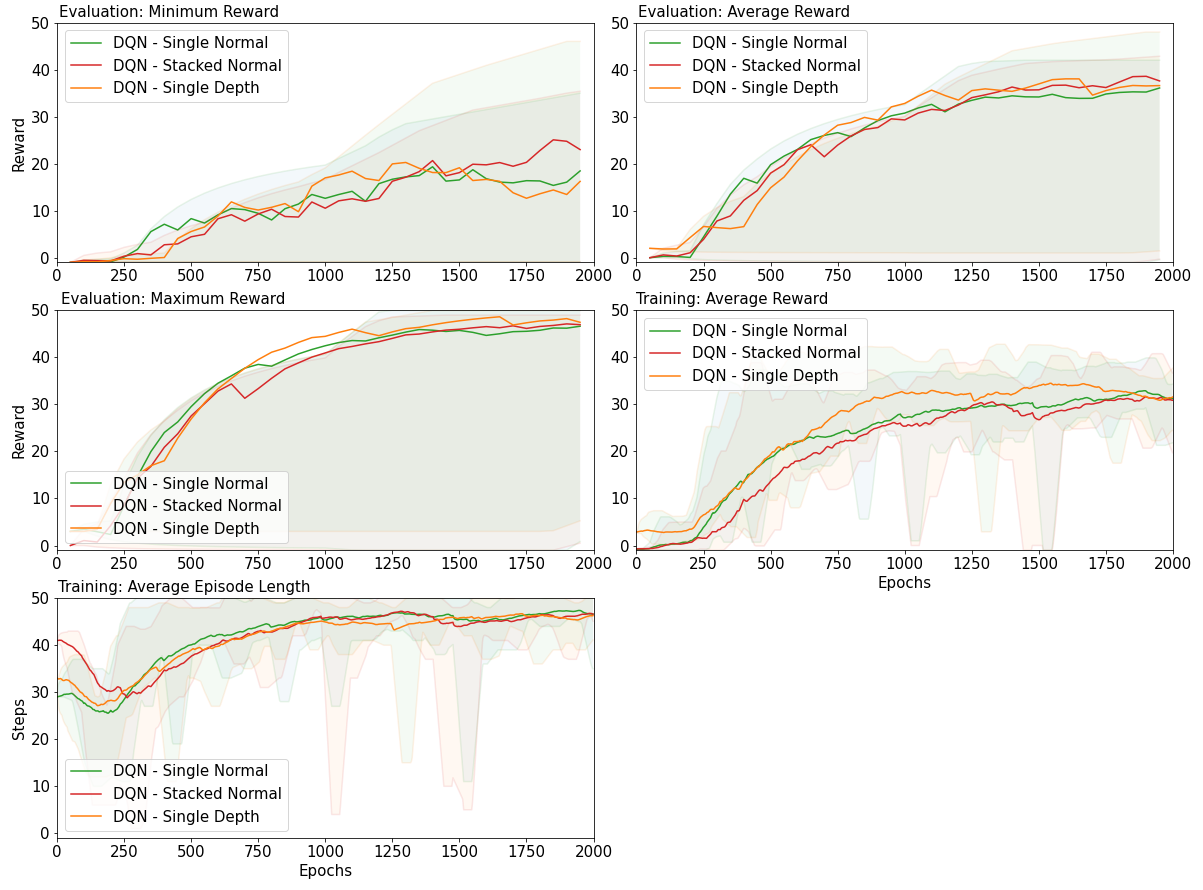
\includegraphics[width=\linewidth]{results/Training for BlocksNormal.png}
    \captionof{figure}{Training Process in BlocksNormal Environment}
    \label{im:NormalTraining}
\end{Figure}

\noindent 
After this, the agent learns better behavior leading to the recovery in the average return.
This dip is not reflected in the average return, because this learning process happens 
before the agent has found the right distances to the person to receive a reward.

Furthermore, during the training process, all the agents were capable 
of converging their average episode length close to the maximum number. Since an episode can 
at most be 50 steps, if the agent is capable of keeping the person in its FoV throughout 
this entire time, the episode length will be 50. Seeing as all the agents are 
able to converge close to this limit, this signifies that the agents have all been able to 
learn how to keep the person in 
their FoV, whatever its distance.
This is reflected 
in the training average return as well, where the curve is similar in shape 
to the average episode length. The longer the episodes, the higher the average rewards that the 
agent is receiving throughout each episode. Being able to 
keep the person in its FoV signifies a first step to learning how to perform the follow-me 
behavior. 

The volatility in the data is explained by the random initialization of the agents. As 
the epochs progress, this volatility reduces, furthermore emphasizing that the agents are 
becoming more stable. 

When it comes to the average return during training cycles, all the agents are able to 
converge to similar values, being around 30. This means that 
out of the 50 steps that the agent is taking, an average of 30 frames were spent in 
goal states. The remaining frames have therefore been spent in states where the person 
was either not centered or not close enough. Comparing this to the evaluation average return, 
this metric converges higher, around 35. The reason 
why this is larger than the training value can be explained with the fact that the 
training cycles happen with a collect policy which includes a certain degree of randomness.
The evaluation cycles are performed using a greedy policy. This means that 
there will always be a slight discrepancy between these two converged values in favor 
of the evaluation average return.  

Looking at the progression of how the agent learned its behavior, 
the maximum value that the agent earned in the evaluation run also converged around 50. 
Therefore, the best episode 
that the agent is able to perform, is one where in most of the steps the agent was 
in a goal state. Considering this, it is interesting to see that the single depth image 
model was able to achieve these near perfect episodes the fastest, compared to the other 
models. The ability to sense the distances between itself and other objects seemed 
to have a positive influence on the training process for the agent in an environment 
where no obstacles are present. 

Finally, the minimum return in an evaluation run is very volatile. This most likely has 
to do with the fact that 
some episodes seem to still confuse the agent enough for it to end the episode very 
quickly by losing it out of sight. Nonetheless, the overall trend of the minimum rewards 
seems to have a positive slope. The final values that all of these agents converge on is 
around 20, which means that the agents have all learned to have a type of behavior that 
at the very least, is able to gather around 20 reward points per episode. 

\subsubsection{Test Results} \label{test_results}
The average return and baseline comparisons of the test runs performed in the BlocksNormal environment can 
be observed in Table \ref{tab:NormalAvgReturn}. 

\begin{table}[H]
    \centering
    \caption{Average return of the agents and performance comparison with the baseline in 
    the BlocksNormal environments}
    \label{tab:NormalAvgReturn}
    \begin{tabular}{l|c|c}
    \textbf{Agent} & \textbf{\begin{tabular}[c]{@{}c@{}}Average return \\ (max. 50)\end{tabular}} & \textbf{\begin{tabular}[c]{@{}c@{}}Compared\\to baseline\end{tabular}} \\ \hline
    Baseline             & 40.2  & -                                                                \\ \hline
    DQN - Single Normal  & 35.2  & -12.43 \%                                                                \\
    DQN - Stacked Normal & 31.9  & -20.64 \%                                                                \\
    DQN - Single Depth   & 42.0  &  +4.5 \%                                                              
    \end{tabular}
\end{table}

Overall, these results show that only some of the RL agents in this environment are able 
to match the performance of the baseline. A surprising result, is that the stacking 
of images did not seem to improve the performance, and had the largest performance 
drop compared to the baseline. This is interesting, as this means that 
although the RL algorithms were able to match the performance of the baseline throughout 
their learning process, the stacked image RL agent did not. Although RL 
is able to teach itself behavior that would be similar to a very straight-forward 
baseline method, the addition of a stacked image state-representation impeded the 
agent so much as to reduce its average return.

Furthermore, the use of depth images instead of normal images did appear to boost the 
agent's performance, enough for an average of 7 frames per episodes and an increase in 
performance compared to the baseline. In order to better understand the behaviors
of each of the RL agents during these test runs, the next sections will focus 
on each specific aspect of their behavior.  \newline

\noindent
\textbf{Reward Distribution} \newline
In order to analyze how each agent performs an average episode and where each agent's 
strongest aspects are, Figure \ref{im:NormalDistro} has been made, 
where the green line represents a running average of the last 5 values.

\begin{Figure}
    \centering
    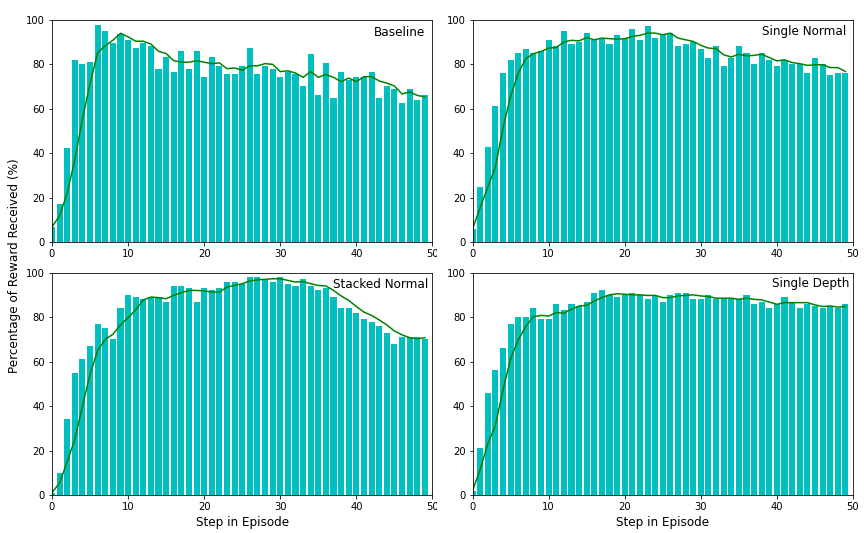
\includegraphics[width=\linewidth]{results/Reward Distribution of BlocksNormal.png}
    \captionof{figure}{Reward Distribution of each agent in BlocksNormal environment}
    \label{im:NormalDistro}
\end{Figure}

As can be seen, there are differences in how each agent performs an average episode. 
Most notable is that, with the exception of the depth agent, most agents struggled with 
keeping a stable reward for longer than 25 steps. Initially, this is not different from the 
baseline and points to the fact that the longer an episode takes, the higher the chance 
the episode ends unsuccessfully. However, the contrast with the depth image is surprising, 
who performs very stable. This shows that the model has learned to 
keep making decisions that allow the agent to stay in goal states on a stable basis.

These results show some 
shortcomings of the RL models which did not use a depth imaging. Both of these agents 
were less stable in their behavior throughout an average episode than the baseline agent. 
In order to analyze what the exact behaviors are that lead to these reward distributions, 
a more in-depth look will be taken at each of them inside of the environment. \newline

\begin{SCfigure}[][h]
    \centering
    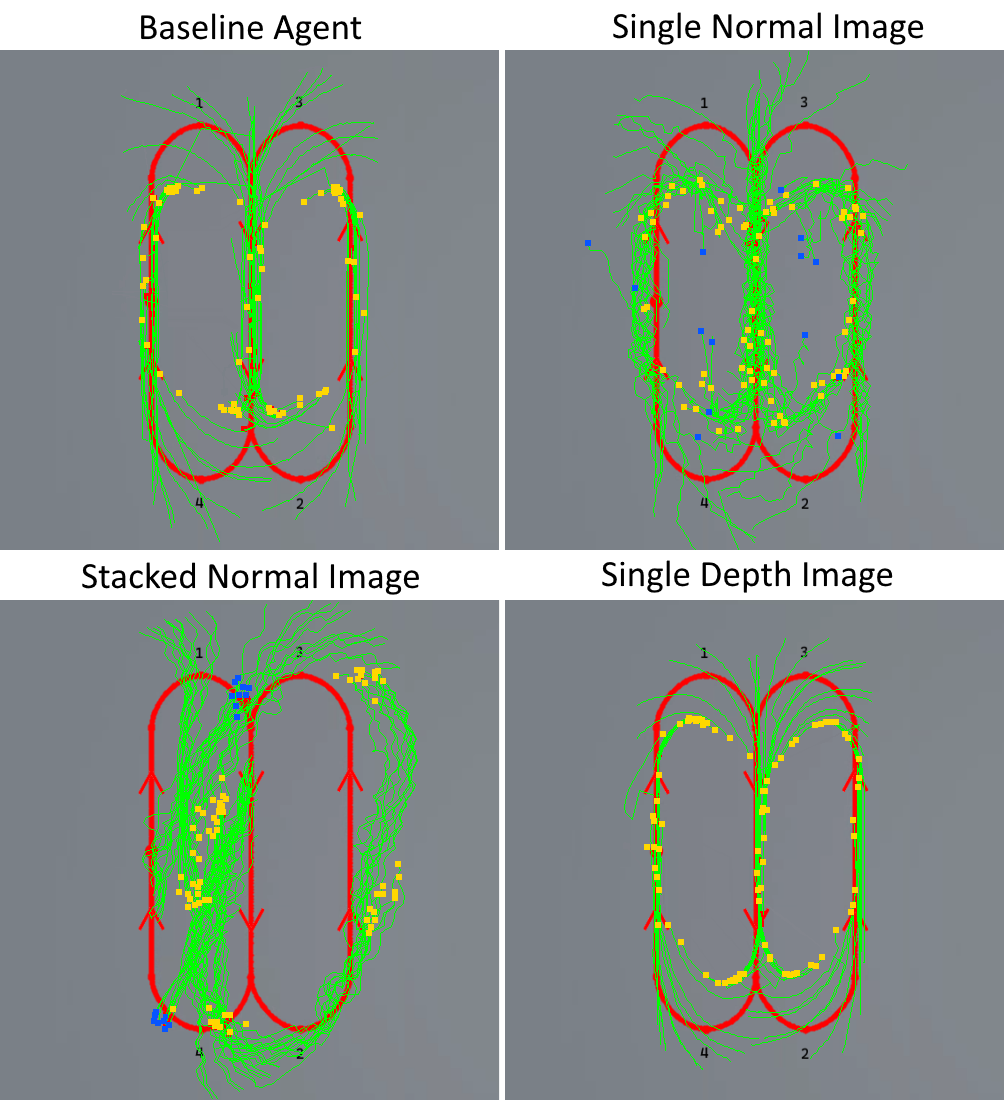
\includegraphics[width=0.66\linewidth]{results/summary-BlocksNormal-Pathsnew.png}
    \captionof{figure}[Paths and episode ends of all the agents during a 100 episode test run in BlocksNormal]{Paths and episode ends of all the agents during a 100 episode test run. 
    The green lines represent the flight paths of the agent.\newline\newline
    The dots correspond to the following episode ends: \newline
    Red = Collisions\newline
    Blue = Out of View \newline
    Yellow = Normal\newline\newline\newline\newline\newline\newline\newline\newline\newline\newline\newline\newline\newline}
    \label{im:NormalPaths}
\end{SCfigure}

\noindent
\textbf{Behavior} \newline
To analyze the overall behavior of the agents, the paths throughout the 100 episode 
test runs have been superimposed over the path of the person. This imposition can be 
seen in Figure \ref{im:NormalPaths}. The added green lines are the path of the agent 
during the episode. The red dots have been the episode ends that occurred through a crash. 
Blue dots indicate the drone lost sight of the person and a yellow dot simply means that the 
episode ended after 50 steps. 

The most notable element in this image, is the contrast that 
the single normal and stacked normal image agents have compared to the 
other two agents. Both of the former agents have very rough flying paths compared 
to the other two. The single normal image has taught itself how to follow the person around its 
paths, but has done so with behavior that is still sub-optimal considering its average return and 
includes a high level of variability. Considering the frequencies of unsuccessful episode ends from 
Table \ref{tab:NormalEnds}, this further emphasizes the weaknesses of this agent. 

\begin{table}[h]
    \centering
    \caption{Out of View of the agents in the BlocksNormal environment during testing}
    \label{tab:NormalEnds}
    \begin{tabular}{l|c}
    \textbf{Agent}       & \textbf{Out of View (/100)} \\ \hline
    Baseline             & 0                           \\ \hline
    DQN - Single Normal  & 15                          \\
    DQN - Stacked Normal & 19                          \\
    DQN - Single Depth   & 0                         
    \end{tabular}
\end{table}

A possible explanation for this high variability could be the fact that the use of 
normal images results in a large state-space making it hard for the 
agent to find a global optimum. Instead, it settles at a local optimum and the search 
for better action sequences remains hard and prone to fail.  

With regards to the other underperforming agent, the stacked normal agent
performs a completely different behavior than 
all of the others. This agent positions itself to the right of the person 
and attempts at keeping the person in view from this perspective. This strategy works 
throughout the moments where the person is walking forward, however, as can be observed 
in Figure \ref{im:normalrun2loses}, it finds itself in a situation that is much more difficult to successfully 
process afterwards. 

\begin{figure}[h]
    \small 
    Image: view of the drone $|$ Arrows: Action the agent performed
    \centering
    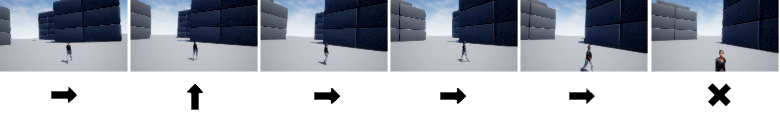
\includegraphics[width=\linewidth]{results/specific_situations/normalrun2-outofview.png}
    \caption{Stacked normal agent losing sight of the person}
    \label{im:normalrun2loses}
\end{figure}

Such situations explains the sudden drop 
in the reward distribution in Figure \ref{im:NormalDistro}, which happen because 
the agent deals with these states in later stages of an episode, as seen in Figure \ref{im:NormalPaths}.

A potential explanation could be the fact that a combination of an increased state-space 
by the stacking of images and the ability to perceive movements better when the drone is 
positioned sideways is impeding the learning process. Positioning itself to the side at 
some point during the training process could lead to higher rewards for the agent. 
Once this behavior has been reinforced through a large number of training cycles, it is 
increasingly hard for the agent to unlearn this behavior. This is especially the case considering 
that the DQN samples from a the larger replay buffer, reinforcing its memory that these 
actions lead to higher rewards. Furthermore, when these sequences of actions lead to 
later situations that are problematic, as seen in Figure \ref{im:normalrun2loses}, the 
increased state-space also impedes the agent even more to find better action sequences. 

Finally, looking at the single depth agent, the higher values in average return 
are being reflected in its behavior. 
The overall flight paths are smooth, even compared to the baseline. Its 
behavior is therefore very stable, further emphasizing its stability as was observed 
in its reward distribution (Figure \ref{im:NormalDistro}). Furthermore, no episode 
has ended in the agent losing sight of the person. 

In contrast to the other agents, the performance of the depth agent points to the simplifying
ability of using a depth map state-space. Additionally, the opposite can be said about the 
use of stacks of images. Increase in state-space in this manner is not helpful, at least in 
environments where they do not convey useful additional information
and the opposite effect with regards to the stacking the state-space. Comparing the agents 
to the baseline, indicates that there 
is a benefit of using RL methods combined with depth maps over the baseline in the task of 
follow-me behavior in an obstacle-free environment. Meanwhile, the use of normal images and 
stacked imaging do not provide useful additions to an agent in this context. 

\subsection{BlocksObstacles Environment}
In this section, a similar procedure
will be performed in the BlocksObstacles environment. Additionally, extra analysis 
regarding the behavior of the agents will be performed to get a grip on the bottlenecks of 
each specific agent. Furthermore, using 
the best working agent from the initial training and test runs, another agent will be 
trained using the same architecture, however with a different reward function. This will 
be performed in order to measure the impact of the reward function on the acquired 
behavior in the context of an environment that contains obstacles. The training 
procedure of all of these agents will be described, which will 
then be followed by the test results of each of them. 

\subsubsection{Training Process}
The training process has proceeded 
very similarly as in the BlocksNormal environment, with some extra points of attention. 
The exact process can be observed in 
Figure \ref{im:ObstaclesTraining}. The most 
notable point that can be seen is that the agents were not able to converge their 
average episode length to the maximum. Some performed better than others however, 
but none of them were able to exceed a 25 step average. An overall trend in all the 
metrics is a significant decrease in performance compared to the previous environment. 
This was to be expected looking at the drop in performance of the baseline in this newer
more complex environment. 

Another interesting point to note is that in the training average metric, we see that 
the stacked depth model was able to get to 
its convergent value the soonest. Especially the single normal image model underperformed 
compared to the other two models, which converged around a similar value. These features 
are also observed in the evaluation average return metrics, where the stacked depth 
image model reached the highest values the quickest. 

Finally, the maximum return of the agents did reach a convergence value of almost 50, 
meaning, again, that the agent's best episodes were the best that the agent could have 
done in these situations. At the same time, the minimum return of the evaluation 
episodes were much lower in comparison to the Blocks training cycle. These features 
show that the models have diverged much more to the extreme, especially in the lower ends, 
which resulted in the reduced performance. It is clear that the obstacles in the 
environment have had a worse effect on the minimum return and not so much on the 
highest return. \newline

\begin{Figure}
    \centering
    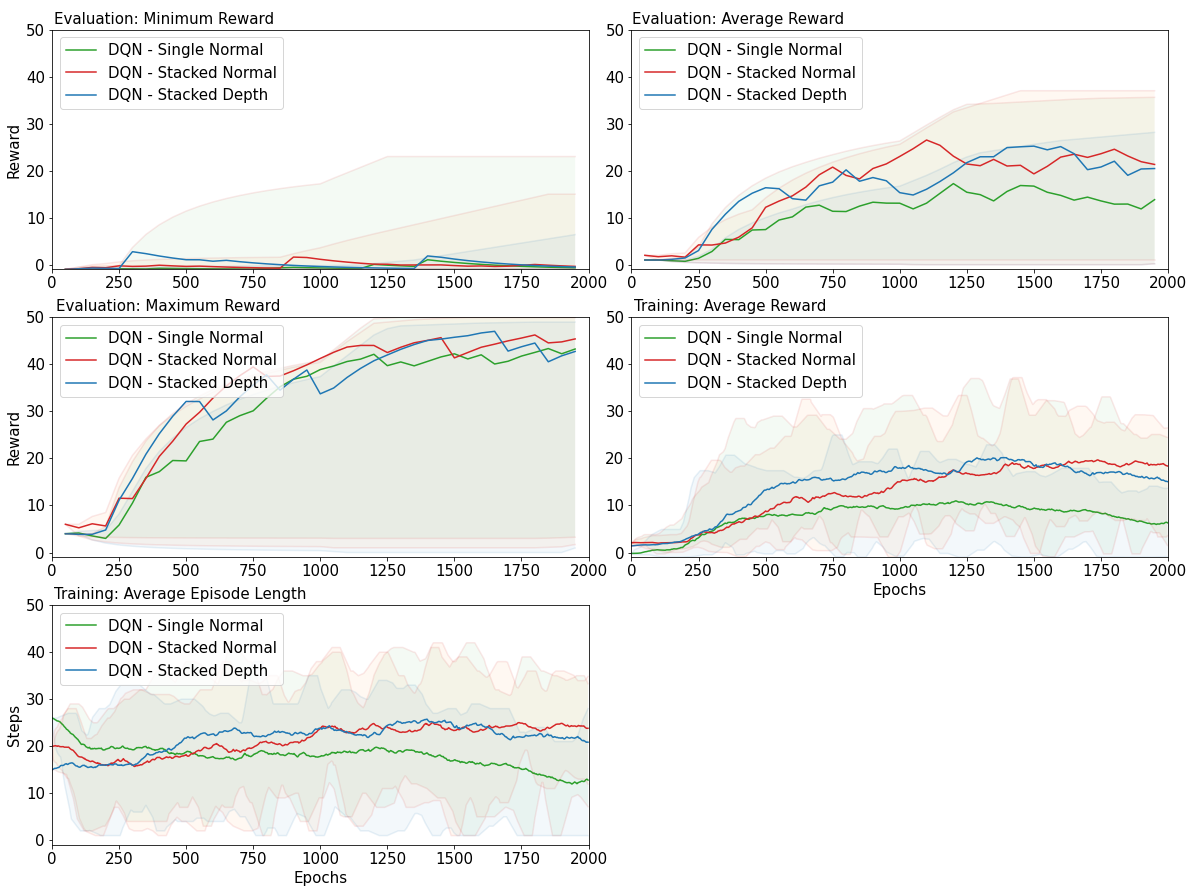
\includegraphics[width=\linewidth]{results/Training for BlocksObstacles.png}
    \captionof{figure}{Training Process in BlocksObstacles Environment}
    \label{im:ObstaclesTraining}
\end{Figure}

\subsubsection{Test Results}
Next, we will look at the results that were obtained from testing the models trained in 
BlocksObstacles environment in their own environment.
The test runs results for this can be seen in Table \ref{tab:ObstacleAVG}. This time, 
the expected return looking at the baseline degradation has also been included and the 
increase in performance compared to the expected return can also be seen. Finally, 
drop in performance compared to the last environment has also been added. 

\begin{table}[h]
    \centering
    \caption{Average return comparisons of test runs in BlocksObstacles}
    \label{tab:ObstacleAVG}
    \begin{tabular}{l|c|c|c|c}
    \multicolumn{1}{c|}{\textbf{Agent}} &
      \textbf{\begin{tabular}[c]{@{}c@{}}Average return\\(max. 50)\end{tabular}} &
      \textbf{\begin{tabular}[c]{@{}c@{}}Expected\\return*\end{tabular}} &
      \textbf{\begin{tabular}[c]{@{}c@{}}Difference\\ expected\\return**\end{tabular}} &
      \textbf{\begin{tabular}[c]{@{}c@{}}Difference\\ previous\\environment***\end{tabular}} \\ \hline
        Baseline             & 22.6 & n.a.   & n.a.  & -43.7 \% \\ \hline
        DQN - Single Normal  & 19.1 & 19.8 & -3.5 \% & -45.7 \%  \\
        DQN - Stacked Normal & 24.8 & 18.0 & \textbf{+37.7 \%} & \textbf{-22.3 \%} \\
        DQN - Stacked Depth   & \textbf{30.1} & 23.6 & +21.6 \% & -28.3 \%
    \end{tabular}
    \justify
    \small
    *The expected return has been calculated by using the degree 
    of degradation of the baseline going from the BlocksNormal to the 
    BlocksObstacles environment. In this case, it was 43.7\%.\newline
    **The percentage change in performance of the agents compared to the expected return. \newline
    ***The performance change for each agent compared to their counterpart in the 
    previous environment. 
\end{table}

These results show that the additions have had a positive influence on the 
performance of each consecutive agent implementation. Most notably, the use of stacked 
images has proven to be a more useful addition to the agent than previously, having 
the largest performance boost compared to the expected performance. Next to this, the 
fact that the performance difference of the stacked normal agent is significantly less than 
the single normal image also emphasizes this point. This is 
the case for both the comparison between the trained agent in the previous environment, 
but also for the comparison to the expected return. Meanwhile, the 
use of depth imaging had even better results. Although the difference has been slightly higher, 
the overall performance is still the highest. Seeing as the depth agents have been the best 
performing models in both environments, this slightly higher performance difference is not unsurprising. 
Overall, the stacked and depth agents outperformed the baseline performance, both 
in expected degradation and average return. 

These results show an initial clue that the use of 
RL algorithms can produce better performing models compared to the baselines. However, 
the state-representation used for these RL agents does matter. Further details will 
be elaborated upon in the next section. The specific behavioral elements that comprise these 
results will be analyzed next.  \newline

\noindent
\textbf{Reward Distribution} \newline
Looking at the rewards that each agent received on an average episode during 
the test run, which can be found in Figure \ref{im:ObstacleDistro}, we see some differences 
between the agent's behavior. 

\begin{Figure}
    \centering
    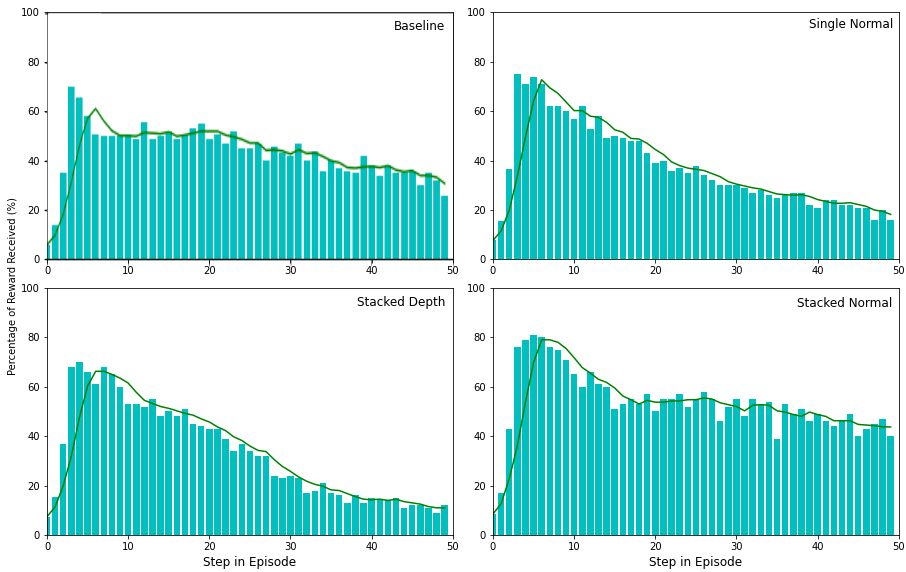
\includegraphics[width=\linewidth]{results/Reward Distribution of BlocksObstacles.png}
    \captionof{figure}{Reward distributions of models trained in BlocksObstacles environment}
    \label{im:ObstacleDistro}
\end{Figure}

The only difference that stacking the 
images does is a slightly larger reward during the intermediate steps of an 
episodes. This means that the agent is in goal states for a longer duration, before 
dropping to the lower values. However, both of these agents, in contrast to the stacked 
depth image model, have a downward trend. The longer the episode, the more 
the agent struggles with follow-me behavior, getting itself in crashes, losing 
sight of the person or simply being too far. However, the stacked depth image model can 
keep a steady value from the 15th frame onwards, despite a drop in the initial frames. 
It is clear that the previously observed stable behavior in the BlocksNormal environment 
is also appearing in this new environment. Again, the use of 
depth maps has been a beneficial aspect with regards to the agents developing overall 
stable behavior. Nonetheless, the 
depth agent still is struggling with later stages in an episode. The behaviors responsible 
for these distributions will be analyzed next.\newline

\noindent
\textbf{Behavior} \newline
The next analysis will look at the flight paths of the agents in the BlocksObstacles environment. 
The visualization for these paths can be seen in Figure 
\ref{im:ObstaclePathsDivided}. Additions to this figure are the areas in which the episode 
ends have taken place. These areas will be used to analyze the specific obstacles and 
situations the agents struggled with. The flight paths without these areas can be seen in 
Figure \ref{im:ObstaclePaths} in appendix \ref{appendixA}. \newline


\begin{SCfigure}[][h]
    \centering
    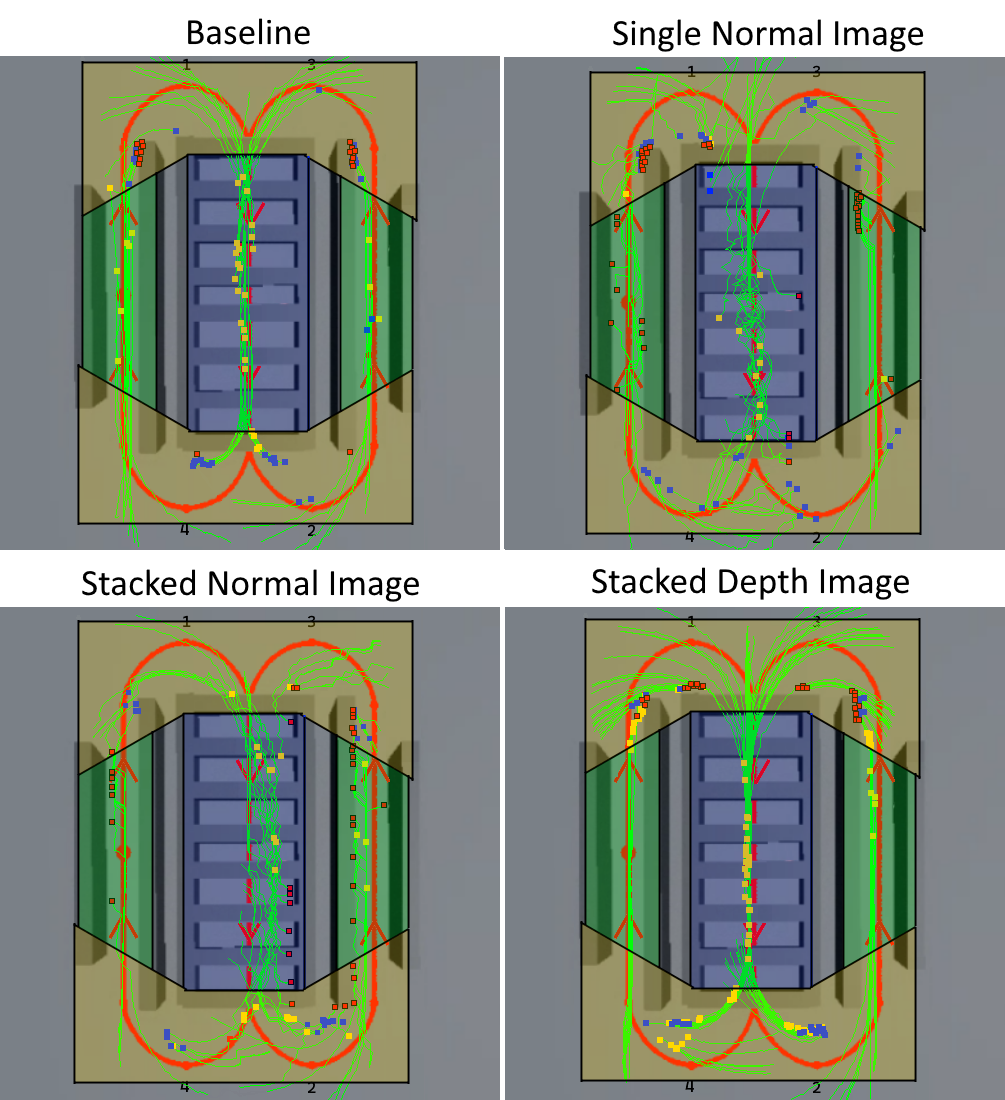
\includegraphics[width=0.66\linewidth]{results/summary-BlocksObstacles-PathsDivision.png}
    \captionof{figure}[Paths and episode ends of all the agents during a 100 episode test run in BlocksObstacles.]{Paths and episode ends of all the agents during a 100 episode test run in BlocksObstacles. 
    The green lines represent the flight paths of the agent.\newline\newline
    The areas correspond to the following situations: \newline
    Green = Tight hallways\newline
    Blue = Wide hallways \newline
    Yellow = Corners \newline\newline
    The dots correspond to the following episode ends: \newline
    Red = Collisions\newline
    Blue = Out of View \newline
    Yellow = Normal\newline\newline\newline\newline\newline\newline}
    \label{im:ObstaclePathsDivided}
\end{SCfigure}

From these images, the erratic behavior of the single normal image is visible again.
Furthermore, the stacked normal agent also repeats the pattern of behavior of 
positioning itself to the side of the person, however this time on the left side. 

Moving on to the next agent, the depth agent, the same pattern of smooth 
and stable flight paths can be observed as previously. Nonetheless, in this 
environment, the number of collisions and out of views has increased, as can 
be observed in Table \ref{tab:ObstacleEnds}. The specific behavior that resulted 
in these numbers will be further analyzed. This will be performed by looking at each 
type of obstacle separately. What ending location corresponded to what area
in this count can be observed in Figure \ref{im:ObstaclePathsDivided}. \newline

\begin{table}[h]
    \centering
    \caption{All of the unsuccesful ends inside of the BlocksObstacles environment test runs}
    \label{tab:ObstacleEnds}
    \begin{tabular}{l|c|c|c|c|c|c|c|c|c}
    \multicolumn{1}{c|}{\textbf{Agent}} &
      \multicolumn{3}{c|}{\textbf{Collisions}} &
      {\ul Total} &
      \multicolumn{3}{c|}{\textbf{Out of View}} &
      {\ul Total} &
      \textbf{\begin{tabular}[c]{@{}c@{}}Total\\ Overall\end{tabular}} \\ \hline
    \multicolumn{1}{c|}{\textit{Obstacle Type}} &
      \textit{Tight} &
      \textit{Wide} &
      \textit{Corners} &
      {\ul } &
      \textit{Tight} &
      \textit{Wide} &
      \textit{Corners} &
      {\ul } &
      \textbf{} \\ \hline
    Baseline       & 0  & 0 & 20 & {\ul 20} & 2 & 0 & 30 & {\ul 33} & \textbf{53} \\
    Single Normal  & 25 & 3 & 18 & {\ul 46} & 0 & 4 & 39 & {\ul 43} & \textbf{89} \\
    Stacked Normal & 17 & 7 & 14 & {\ul 38} & 0 & 0 & 24 & {\ul 24} & \textbf{62} \\
    Stacked Depth  & 0  & 0 & 25 & {\ul 25} & 0 & 0 & 24 & {\ul 24} & \textbf{49}
    \end{tabular}
\end{table}

\noindent
\textit{Hallways} \newline
The two types of hallways will be discussed further, starting with the wider hallway.
This type of situation has been comparatively the easier obstacle to deal with by 
the agents. Here, the only agents that have had problems have been the normal image 
agents. The fluctuant pattern of the single normal agent results in a sporadic end where 
it crashed against the wall. However, the other times the agent crashes or loses the person, 
it is as a 
run-up to the oncoming turn of the person. Looking at the flight patterns in 
Figure \ref{im:ObstaclePaths}, these mishaps are the results of the overall volatile 
behavior that this agent exhibits and not of a specific behavior pattern that was learned 
by the agent. 

Adding stacked images to this agent has shown the number of 
crashes in the wider hallway situation to be increased, while the times 
it lost sight of the person brought to zero. Looking at the flight 
patterns of this agent, much as in the previous environment, 
it clearly has a tendency to position itself to the side of the person. However, this time 
to the left. This, unfortunately, positions the drone in such a way that the walls are not 
visible anymore and a crash occurs. One such situation can be seen in Figure \ref{im:run2crashes}.

\begin{Figure}
    \centering
    \small
    Image: view of the drone $|$ Arrows: Action the agent performed
    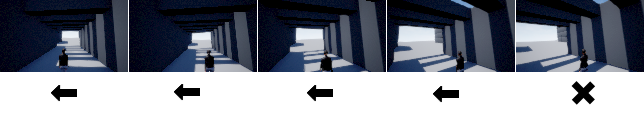
\includegraphics[width=\linewidth]{results/specific_situations/ObstaclesRun2-collision.png}
    \captionof{figure}{How the stacked normal agent crashes into the wall from behind}
    \label{im:run2crashes}
\end{Figure}

This behavior is a continuation of the problems during the learning process that was 
described in the previous section and is probably explained by a similar interpretation.
However, a possible explanation for why this time the preferred side of the agent to position 
itself differs, is a random choice early in the learning process. Developing this behavior 
early in the training process, an initial choice about which direction to go is made randomly.
It is then hard to unlearn this behavior, as mentioned earlier, because of the replay 
buffer sampling of the DQN. 

Looking at the tighter hallways, these situations have been a more difficult setting for some 
of the agents to 
deal with. Again, a similar division of the agents can be perceived, where the normal 
image agents have the most trouble with this situation, and the baseline and 
depth agent had no problems at all. For the two problematic agents, the pattern of 
behavior that leads to these failed endings are similar to those in the 
wider hallway. The increase in frequencies can be explained by the fact that 
the hallway is tighter, bringing about these situations sooner and more often. 
The baseline, which follows the path of the person very tightly, logically did not 
struggle with this situation. However, interesting to note is that this type of 
following is not achieved by the normal image agents, but has been by the depth 
agent, as reflected in the table. These findings additionally reinforce the 
hypothesis that the depth state-space allows for easier learning of behavior 
compared to the grayscale state-space. On top of that, the use of stacked state-
representation seems to ba a valuable addition in some contexts. Here, the 
environment and the type of pixel value matters.   \newline

\noindent
\textit{Corners} \newline
With regards to the corner situations, the variations to the agents proved to be 
useful additions that allowed them to better avoid the obstacles. 
However, the ability to perform significantly better than the baseline in this aspect is 
not observed. The single normal image had trouble completing 
any episode successfully, as can be seen in Table \ref{tab:ObstacleEnds}, 
struggling the most with corners, where a large portion of the collisions 
and out of view endings happened. This effect likely explained 
by the high volatility of its behavior that results in many different types of 
episode ends and beginnings. Overall, these results more strongly emphasize 
the problems of using single normal images as a state-representation, especially 
compared to the other agents. What's more, this agent does not show clear 
advantages over using the baseline method.  

The stacked agent was recorded having significantly less 
endings where the drone lost sight of the person. The number of times 
that a collision has occurred has decreased, but not by a large margin. This 
is explained by the fact that instead of having trouble in multiple places, the 
agent now is struggling at more specific moments, which in this case is the moment 
halfway through a turn. An example of the agent in this 
situation can be seen in Figure \ref{im:run2loses}. 

\begin{Figure}
    \centering
    \small
    Image: view of the drone $|$ Arrows: Action the agent performed
    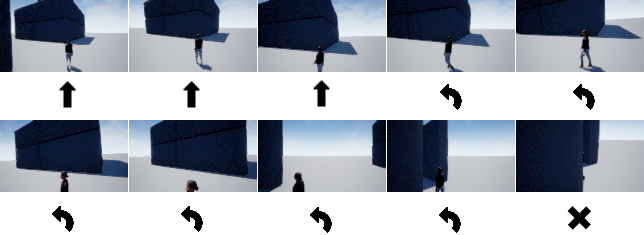
\includegraphics[width=\linewidth]{results/specific_situations/obstaclesrun2-outofview.png}
    \captionof{figure}{How the stacked normal agent loses the person}
    \label{im:run2loses}
\end{Figure}

It is apparent that the agent is upholding the behavior of following the person from the 
left. In some cases, it allows the drone to pass the first corner but holding on 
to this behavior leads to the problem of being blindsided 
by the wall that is appearing moments later. When in the situation of the last two 
frames of the figure, the agent is too close and unable to correct is behavior on time before 
losing sight of the person. In the clusters in the bottom left turns, the antithesis to this 
behavior is visible. Here the drone is too far away from the person to handle the final stages 
of the turns, resulting in losing the person. Finally, the top two turns have their own 
clusters, but in these situations, collisions are more apparent. This difference is 
because in the bottom turns, the drone is coming out of the 
wider hallway, which lends more space to position itself accordingly. In the top, 
the drone is coming out of the tighter hallway, lending less space for such manoeuvers. 
These results show that the stacking of images helps the agent in overall performance, meaning 
that the agent spends more time in goal states compared to the previous implementation. However, 
significant improvement in performance compared to the baseline is missing, and the increase in 
unsuccessful episode ends emphasize shortcomings in the learned behavior. 

Finally, the depth agent was struggling exclusively in the 
corners, mimicking the baselines behavior much more. As can be seen, in the top 
two corners, the agent has clusters of crashing, while in the lower two it is exclusively 
losing sight of the person. Again, this difference is explained by drone exiting either a 
wide or tight hallway. The baseline exhibits the same behavior. However, an interesting 
difference, is that the stacked depth agent has taught itself to position itself much 
closer to the person, as can be seen in Figure \ref{im:run3loses}. 

\begin{Figure}
    \centering
    \small
    Image: view of the drone $|$ Arrows: Action the agent performed
    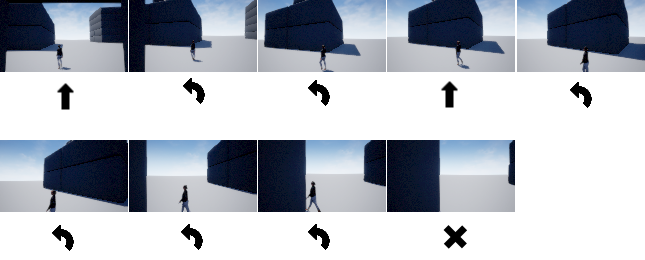
\includegraphics[width=\linewidth]{results/specific_situations/obstaclesrun3-outofview.png}
    \captionof{figure}{How the stacked depth agent loses the person}
    \label{im:run3loses}
\end{Figure}

It does so especially during the moments where the turn is occurring, in 
order to move past the first wall, so that it can focus on centering the person in its view. 
However, the issue is that after this has been done, the person is walking towards the 
second corner, which the drone is unable to see and correct for on time. 
What is interesting about this behavior is that it shows the ability of the agent to 
learn how to navigate itself around the first corner. It is struggling 
with the second stage of this process, because it is unable to observe the wall 
in order to act on time. These patterns are furthermore emphasized by the comparison of 
the flight paths seen in Figures \ref{im:ObstaclePathsDivided} and \ref{im:NormalPaths}.
For the general flight paths, Figure \ref{im:ObstaclePaths} in appendix \ref{appendixA} 
can be consulted. 

Interestingly, when looking at the flight paths of the depth agent in this environments 
compared to the BlocksNormal environments, it appears that the shape 
is different. The shape is clearly correcting for the obstacles 
in the former environments. It is unfortunately not always able to successfully finish 
this route, but the behavior does show that the agent is aware of the structures and 
has taught itself behavior to avoid it, albeit not completely infallible. 

A possible reason for why these situations are still so hard for the agent to deal with, 
could relate to shortcomings of the DQN agent. Considering the fact that DQNs 
are implemented using a memory buffer, they sample from their memory during the 
entire learning process. Seeing as most of the time, the person is walking 
straight, the largest proportion of experiences in the training batch will include 
transitions where the person is walking straight. Overall, this creates a bias 
in this replay buffer towards straight walking experiences, making it much harder 
for the agent to learn what to do with the turns. Nonetheless, compared to the 
baseline, these results have shown promising results for the capabilities of RL 
agents to learn behavior to avoid obstacles. \newline


\subsection{Warehouse Environment} \label{warehousetest}
The final environment in which tests have been performed, is the Warehouse environment. 
Here, the best performing agent from each environment is tested. Since these had 
different state-representation, the better working version of these agents in the Warehouse 
environment test runs will be retrained inside of this environment. 

\subsubsection{Training Process}
After the tests runs have been performed, for which the results and their corresponding 
elaboration can be seen in Section \ref{warehousetest}, the best performing model 
was the stacked depth model. The training process for this agent can be observed in 
Figure \ref{im:WarehouseTraining}.

\begin{Figure}
    \centering
    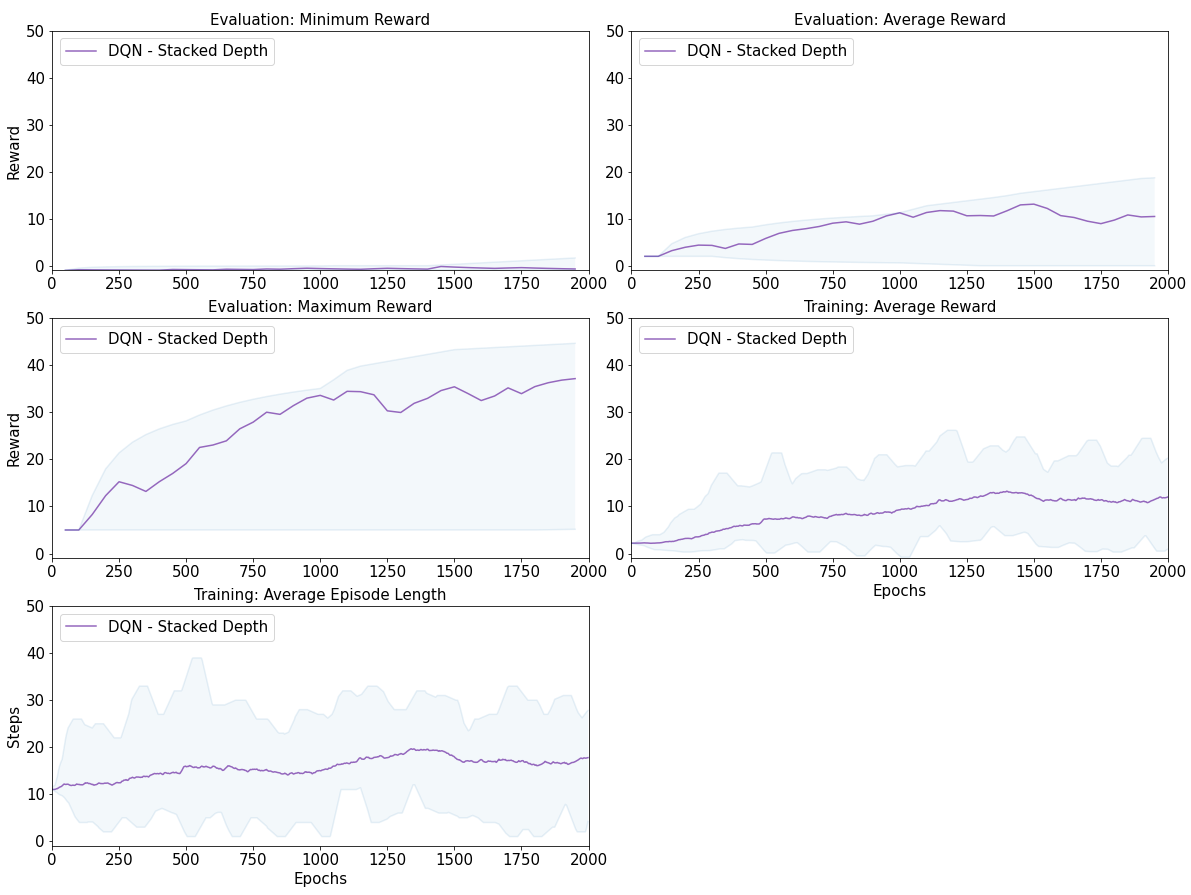
\includegraphics[width=\linewidth]{results/Training for Factory.png}
    \captionof{figure}{Training of Stacked Depth agent in Warehouse}
    \label{im:WarehouseTraining}
\end{Figure}

The results for the training of the stacked depth agent inside of the warehouse environment 
show a similar degradation in training performance as was perceived in the BlocksObstacles 
environment compared to the BlocksNormal. However, the degree of this degradation in this 
environment is lower. The average episode length during training time converged around a 
similar value than the BlocksObstacles environment, which was around 20 steps. 
Furthermore, both the average return during training time and evaluation time converged around 
a value of 10. These are only marginally lower than their counterparts in the BlocksObstacles 
environment, being 10 and 20 respectively. This is most likely cause by a lower minimum return, 
being almost never higher than zero. Next to this, the maximum return is also lowered, 
not reaching the maximum score of 50. 
The complexity of the environment has added increased difficulty for the learning process 
of the agent. The test results will elaborate on whether this also has an impact on the 
degree to which the agent behaves inside of the environment compared to other agents. 

\subsubsection{Test Results}
The final tests that have been performed all focus on the generalizability of 
RL agents to a new, more complex environment. This will be performed by using 
the degradation in performance that was observed in the baseline performing 
in the new environment. This drop in performance of the baseline is compared 
to the trained DQN - single depth agent in the BlocksNormal environment, the 
trained DQN - stacked depth agent in the BlocksObstacles, and a retrained DQN - 
stacked depth agent in the Warehouse environment. The average returns and the
compared performance drops can be observed \ref{tab:WareAVG}. 

\begin{table}[h]
    \centering
    \caption{Average return comparisons for the test runs in the Warehouse environment}
    \label{tab:WareAVG}
    \begin{tabular}{l|c|c|c|c}
    \multicolumn{1}{c|}{\textbf{Agent}} &
    \textbf{\begin{tabular}[c]{@{}c@{}}Average return\\(max. 50)\end{tabular}} &
    \textbf{\begin{tabular}[c]{@{}c@{}}Expected\\return*\end{tabular}} &
    \textbf{\begin{tabular}[c]{@{}c@{}}Difference\\ expected\\return**\end{tabular}} &
    \textbf{\begin{tabular}[c]{@{}c@{}}Difference\\ previous\\environment***\end{tabular}} \\ \hline

        Baseline                  & 9.9   & --  & -- & -56.2 \%       \\ \hline
        (Normal) Single Depth     & 11.5 & 11.5 &  0 \% & -72.7 \%     \\
        (Obstacles) Stacked Depth & 13.8 & 13.1 & +5.3 \% & -54.1 \%  \\
        (Warehouse) Stacked Depth & 21.6   & -- & +64.9 \% & -28.3 \%

    \end{tabular}
    \justify
    \small
    *The expected return has been calculated by using the degree 
    of degradation of the baseline going from the BlocksNormal to the 
    BlocksObstacles environment. In this case, it was 56.2\%.\newline
    **The percentage change in performance of the agents compared to the expected return. \newline
    ***The performance drop for each agent compared to their counterpart in the 
    previous environment. 
    \end{table}

Unsurprisingly, the baseline was the most underperforming agent of the set. However, 
the transferred agents, from both environments, only improved slightly. This is 
especially visible when compared to the expected return according to the degradation 
of the baseline. The single depth agent, trained in BlocksNormal, showed the exact 
amount of performance degradation as the baseline. Furthermore, the BlocksObstacles 
trained agent only improved slightly compared to the expected results. Nonetheless, 
the performance drop compared to their trained environments, can be seen to be the 
lowest for the BlocksObstacles trained agent. Nonetheless, the newly 
trained agent had the overall better performance. The added complexity of the 
obstacles formed a much larger problem for single depth agent. These results 
suggest that there has been little transfer of knowledge to the new domain. 
However, to further confirm these findings, a more in-depth look will be taken 
at their specific behavior. 


\begin{SCfigure}[][h]
    \centering
    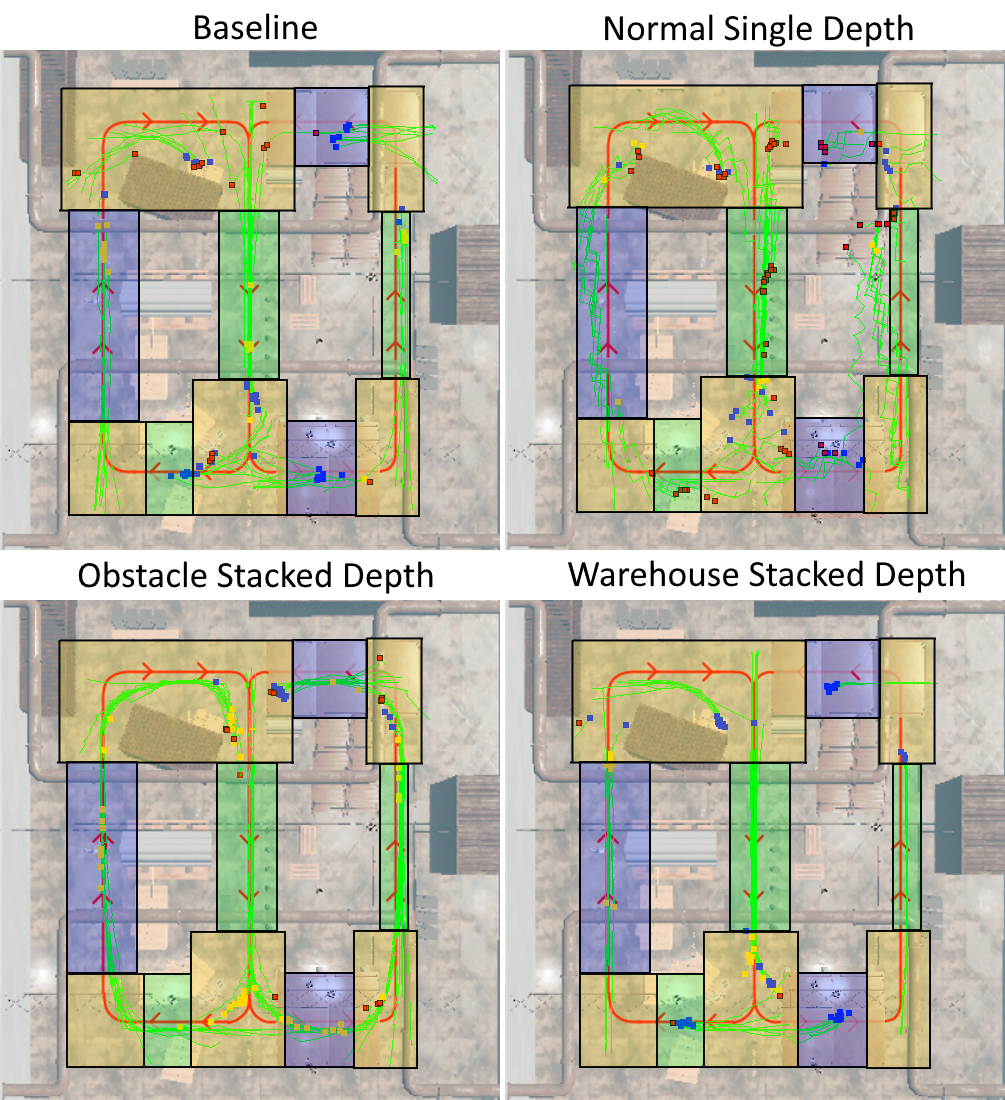
\includegraphics[width=0.66\linewidth]{results/WarehousePathsDivision.png}
    \captionof{figure}[Paths and episode ends of all the agents during a 100 episode test run in the Warehouse environment. ]{Paths and episode ends of all the agents during a 100 episode test run in the Warehouse environment. 
    The green lines represent the flight paths of the agent.\newline\newline\newline\newline\newline\newline\newline\newline
    The areas correspond to the following situations: \newline
    Green = Tight hallways\newline
    Blue = Wide hallways \newline
    Yellow = Corners \newline\newline
    The dots correspond to the following episode ends: \newline
    Red = Collisions\newline
    Blue = Out of View \newline
    Yellow = Normal}
    \label{im:FactoryPathsDivided}
\end{SCfigure}

Visible in Figure \ref{im:FactoryPathsDivided} is the fact that the depth images trained in environments with 
obstacles, showed the similar stable behavior that was observed in the previous 
two experiments, is visible in this one as well. However, what is interesting, is the 
fact that the agent trained in BlocksNormal was much more erratic. More surprisingly, 
is that a similar behavior that was observed in the stacked normal image agents, 
is now visible in this agent. The agent is trying to position itself to the left of 
the person throughout the episodes. This results in the increased crashes and 
out of views that is visible in Table \ref{tab:WareEnds}. This behavior 
only being expressed in this environment, is a sign that the agent is confused 
with the state-space. Not having been trained on any state that included obstacles, 
now clearly shows to be a problem for the agent in 
spaces where there are objects. This perturbs the agent so much as to illicit this unusual
behavior, with a bias towards the "move left" action. This shows that there is a limit to 
the generalizability 
capabilities of RL. Not having seen any instances of a given situation renders the agent 
incapable of acting accordingly. This explains the minimal 
transfer of its behavior to this new environment, as seen in Table \ref{tab:WareAVG}.
Further emphasizing this point, is Table \ref{tab:WareEnds}.

\begin{table}[h]
    \centering
    \caption{All of the unsuccesful ends inside of the Warehouse environment test runs}
    \label{tab:WareEnds}
    \begin{tabular}{l|c|c|c|c|c|c|c|c|c}
    \multicolumn{1}{c|}{\textbf{\begin{tabular}[c]{@{}c@{}}Agent\\(trained in:)\end{tabular}}} &
      \multicolumn{3}{c|}{\textbf{Collisions}} &
      {\ul Total} &
      \multicolumn{3}{c|}{\textbf{Out of View}} &
      {\ul Total} &
      \textbf{\begin{tabular}[c]{@{}c@{}}Total\\ Overall\end{tabular}} \\ \hline
    \multicolumn{1}{c|}{\textit{Obstacle Type}} &
      \textit{Tight} &
      \textit{Wide} &
      \textit{Corners} &
      {\ul } &
      \textit{Tight} &
      \textit{Wide} &
      \textit{Corners} &
      {\ul } &
      \textbf{} \\ \hline
    Baseline       & 0  & 1 & 15 & {\ul 16} & 5 & 13 & 42 & {\ul 60} & \textbf{76} \\
    BlocksNormal & 21 & 8 & 27 & {\ul 56} & 0 & 5 & 51 & {\ul 38} & \textbf{94} \\
    BlocksObstacles & 0 & 0 & 22 & {\ul 22} & 0 & 0 & 25 & {\ul 25} & \textbf{47} \\
    Warehouse & 1  & 0 & 2 & {\ul 3} & 11 & 12 & 45 & {\ul 68} & \textbf{71}
    \end{tabular}
\end{table}

What is interesting to see is that the two stacked depth agents performed better, but
their results are mixed. The stacked depth agent trained in the BlocksObstacles environment 
scored a lower average return, but had much less unsuccessful episode ends. These 
two results contradict each other. What seems to happen is that the retrained agent 
had much more trouble with not losing the person in the corners. Looking at the behavior, 
it is clearly visible that the agent is following the person much more closer than 
in the previous environment, as can be seen in Figure \ref{im:factorystackcomesclose}. 

\begin{Figure}
    \centering
    \small
    Image: view of the drone $|$ Arrows: Action the agent performed
    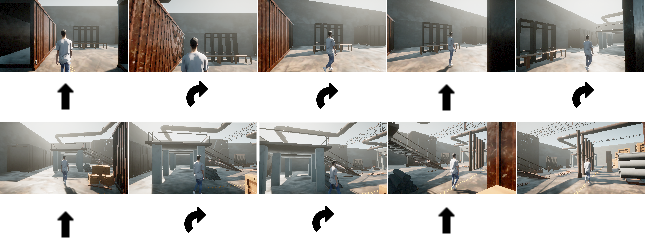
\includegraphics[width=0.9\linewidth]{results/specific_situations/obstaclerun3-comesclose.png}
    \captionof{figure}{How the stacked depth agent comes very close}
    \label{im:factorystackcomesclose}
\end{Figure}

This behavior is much more helpful with avoiding crashes and keeping the person in 
its FoV, however, it is not helpful for receiving reward, as is reflected in its 
average return. This is not reflected in the behavior of the stacked depth that 
has been retrained in the warehouse environment. However, this agent is impeded 
by the fact that it has not learned how to deal with these obstacles accordingly 
and keeps losing the person from its view. It has, however, taught itself to 
to avoid crashes, suggesting its ability to sense the obstacles and 
avoid them enough to not crash. Looking at the distribution of unsuccessful episode ends, 
both agents were 
mostly struggling in the situations of corners. The difference 
between the agents in the other two situations stems from the fact that the 
BlocksObstacles trained agent is closer to the person, leading to failed ends 
closer to the corners. On the other hand, the retrained agent is much farther 
and is therefore failing in similar situations nonetheless. 
These differences show that the best approach is 
still to train an agent in a specific environment. Doing this gives an agent 
the familiarity with the relevant situations to be able to behave accordingly. 
Nonetheless, transferring this knowledge from different environments still shows 
promising results, as the transferred agent behaved quite similarly as it had in 
the previous environment. Emphasizing this even further, is the fact that compared to the 
baseline, both agents performed significantly better. 

\subsection{Reward Functions Comparison}
In the final test, the reward function has been slightly adjusted as described in Section \ref{experiments}.
Using the best working agent from BlocksObstacles, which was the DQN - stacked depth agent, 
a new agent was trained using this new reward function. This reward function was a slight 
decrease in goal states. By making the margins of the goal distances to the 
person smaller, the reward function is made stricter. The overall reward function is thereby made even 
sparser. Testing this newly trained agent will give insights into the effect of the reward 
function on the acquired behavior. 

\subsubsection{Training Process}
The training process of this agent, as can be seen in Figure \ref{im:NewRewardTraining} in 
Appendix \ref{appendixA}, has proceeded almost identical to the training of the same agent 
using the normal reward function. These results are unexpected seeing as the reward function 
has been made even sparser. Seeing as there are even less states in which the agent receives 
a positive reward, it would be increasingly hard for the agent to find its way to these 
goal states. Considering this, the rewards should be overall lower, as the complexity of the 
problem has increased. Nonetheless, it appeared to converge at exactly the same values. These 
results potentially show that the agent learned the exact same behavior as before, leading 
to the similar learning results. This will analyzed below. 

\subsubsection{Test Results}
Having trained the agent using a new reward, a comparison can be made the 
same agent trained using the normal reward. This comparison can be seen in Table 
\ref{tab:RewardAVG}. 

\begin{table}[h]
    \centering
    \caption{Average return of the retrained agent with an adjusted reward function}
    \label{tab:RewardAVG}
    \begin{tabular}{l|c|c}
    \multicolumn{1}{c|}{\textbf{\begin{tabular}[c]{@{}c@{}}Reward \\ function\end{tabular}}} &
      \textbf{\begin{tabular}[c]{@{}c@{}}Average return\\ (max 50)\end{tabular}} &
      \textbf{Difference*} \\ \hline
    Normal Reward &
      39.1 &
      +65.7 \% \\
    Adjusted Reward &
      30.2 &
      --
    \end{tabular}
    \justify
    \small
    *The difference is calculated considering the expected reward for the Stacked Depth model as referenced 
    in Table \ref{tab:ObstacleAVG}. This expected reward was 23.6. 
\end{table}

This table shows that testing the agent using the adjusted reward has given a similar 
reward as the agent trained with a normal reward (Table \ref{tab:ObstacleAVG}). What is 
interesting, however, is that when testing this agent using the normal reward function, 
the average return is much higher. Seeing this increase by itself is not a surprising 
result, considering as the adjusted reward is much more strict compared to the normal 
one. These results show that the more precise a reward function is, the more focussed the 
agent becomes in keeping in these goal states. This is beneficial seeing as normally 
sparse reward functions make the learning process harder, decreasing reward. Important 
to note, is that there is a behavioral change, showing that although the training 
process was similar, the agents have learned different behaviors, which will 
be analyzed next. 

Looking more specifically at an average episode in Figure \ref{im:RewardDistro}, 
it is clear that this agent is better able to maintain the original level of 
rewards received in the early stages of the episode. 

\begin{Figure}
    \centering
    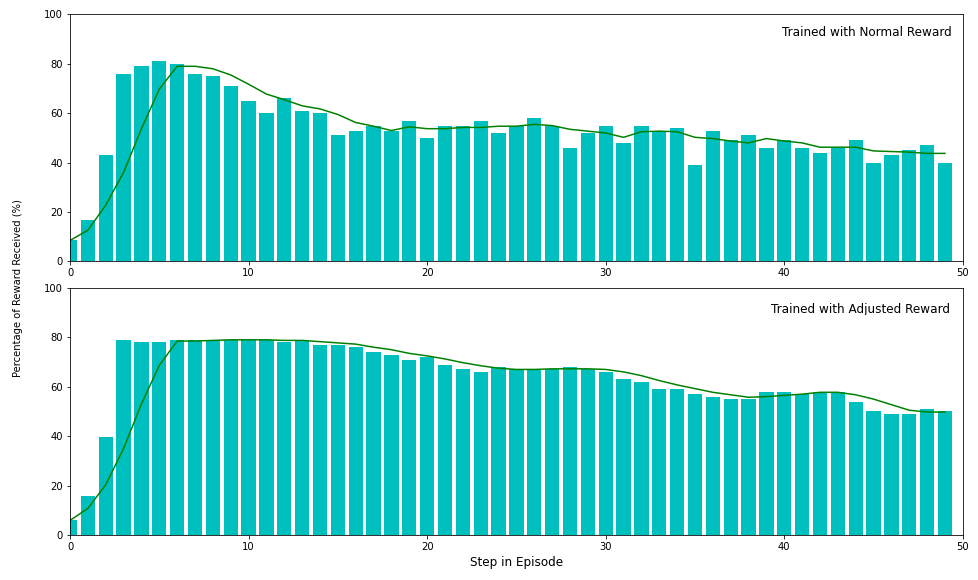
\includegraphics[width=0.8\linewidth]{results/Reward Distribution of NewRewards.png}
    \captionof{figure}{Reward Distribution of agent trained in BlocksObstacles with adjusted reward function.
    The collected rewards have been measured using the normal reward function.}
    \label{im:RewardDistro}
\end{Figure}

Next to this, the decreasing 
trend afterwards is less apparent than the agent trained using a normal reward. It is 
in these initial stages especially that this agent is earning more rewards compared to 
the normal agent. How this is achieved with behavior can be observed in Figure \ref{im:RewardPaths}. 

\begin{SCfigure}[][h]
    \centering
    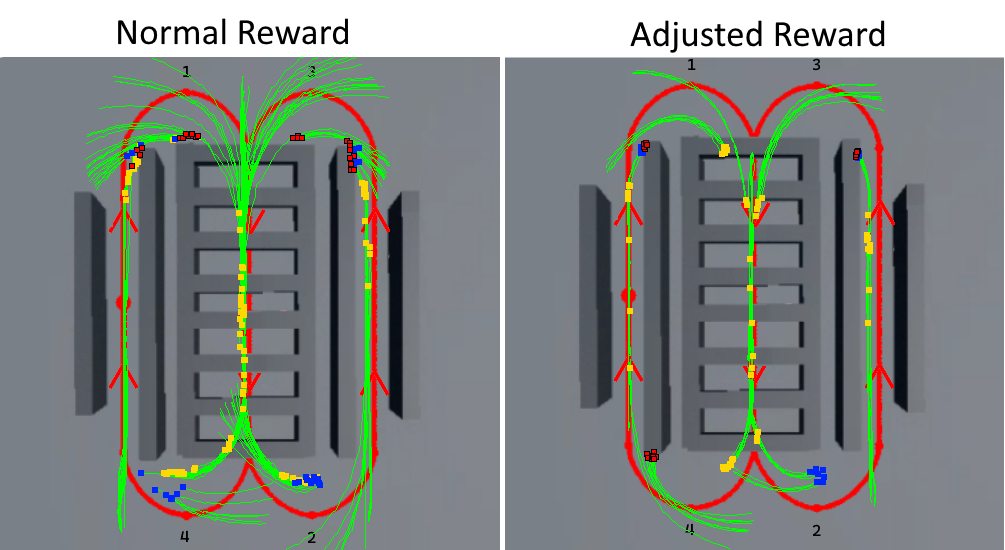
\includegraphics[width=0.66\linewidth]{results/BlocksObstacles Adjusted Rewards Paths.png}
    \captionof{figure}[Locations of each type of situation in the environments]{Locations of each type of situation in the environments\newline\newline\newline\newline
    The dots correspond to the following episode ends: \newline
    Red = Collisions\newline
    Blue = Out of View \newline
    Yellow = Normal}
    \label{im:RewardPaths}
\end{SCfigure}

As can be seen, the overall behavior seems similar. Many of the earlier mentioned behaviors
are apparent again, namely: keeping a stable flight path; staying close to the person's 
walking route; and having no trouble with the hallways situations. These aspects are further 
emphasized by the frequencies of unsuccessful episode ends as seen in Table \ref{tab:RewardEnds}.

\begin{table}[h]
    \centering
    \caption{Episode ends for the same agent trained using two different reward functions in BlocksObstacles}
    \label{tab:RewardEnds}
    \begin{tabular}{l|c|c|c}
    \textbf{Agent trained using:} & \textbf{Out of View} & \textbf{Collisions} & \multicolumn{1}{l}{\textbf{Total (/100)}} \\ \hline
    Normal Reward                 & 24                   & 25                  & 49                                        \\
    Adjusted Reward               & 21                   & 21                  & 42                                       
    \end{tabular}
\end{table}

However, a difference between the agents, is that the agent trained using 
the adjusted reward had overall less unsuccessful episode ends than before. However, 
what is more interesting, is the exact location in which these unsuccessful ends 
have happened. For the agent trained with the normal reward, there were multiple 
corners that were problematic. With collisions and out of view clusters at both 
the start and ending of the turn. However, this agent specifically had problems with 
the entrances and exits of the tight hallways. As can been seen in Figure \ref{im:RewardPaths}, 
the agent trained using the restrictive reward function mostly had collisions 
in the top two turns, in the first stages of exiting the tight hallway. An explanation 
for why it is struggling here is similar as in the BlocksObstacles environment. 
Leaving the tight hallways is hard as there is less room and the agent needs to 
explicitly move around it, which is a harder task in this situation than leaving the wider 
hallway. Next to this, entering the tight hallway is also a problem for the agent, seeing 
as there is another cluster of collisions in the bottom left turn. 

A positive point, nonetheless, is the fact that this agent is not struggling with the rest 
of the turn. This shows that the agent has learned to perform the rest of the turn successfully.
This is an improvement compared to the agent trained using the normal reward, as this agent 
had trouble with both corners in the top turns. Making sense of this, the agent has taught 
itself to follow the person much more tightly than the previous agents. Such behaviors 
are advantageous in situations where there is more room to make the turns. However, 
they also pose problems in the situations where there is no such room. It is apparent that 
the agent struggles more in these situations, and less in these others. This juxtaposition 
nonetheless shows an improvement in overall performance, and only a slight improvement in the
unsuccessful episode ends. Overall, however, this reward function has been a beneficial 
addition to the learned behavior of the agent. 

Concluding, changes to the reward function have a strong influence on the learned behavior. 
Considering the results of this experiment, minimal changes to the reward functions improved 
the behavior significantly. These findings further reinforce the aforementioned concepts that 
the reward signal is the foundation for the learned behavior of an RL agent. Other 
tests with the possibilities of different reward functions are still required, but are 
out of the scope of this thesis. 









